%% =====================================================================
%% paper2/main.tex -- Saturation-aware certification of active chatter
%%                    control: implementation-exact admissible sets,
%%                    causal saturation islands, and the collapse of the
%%                    linear controller ranking.
%% Class: elsarticle, numbered references (refs.bib).
%% Compile: pdflatex main && bibtex main && pdflatex main && pdflatex main
%% Every number in this draft is generated by the repository campaign
%% (results/*.json) -- provenance in docs/paper2_foundational_text_final.md.
%% =====================================================================
\documentclass[preprint,12pt]{elsarticle}

\usepackage{amsmath}
\usepackage{graphicx}
\usepackage{booktabs}

\newcommand{\hinf}{\ensuremath{H_\infty}}
\newcommand{\dz}{\mathrm{dz}}
\newcommand{\Oinf}{\ensuremath{\mathcal{O}_\infty}}
\newcommand{\um}{\,\ensuremath{\mu\mathrm{m}}}
%% Author-side to-do marker (must be empty at submission).
\newcommand{\todo}[1]{\textbf{[TODO: #1]}}

\journal{Mechanical Systems and Signal Processing}

\begin{document}
\begin{frontmatter}

\title{Saturation-aware certification of active chatter control:
implementation-exact admissible sets, causal saturation islands, and
the collapse of the linear controller ranking}

% TODO: final author list, affiliations, ORCID iDs, corresponding author.
\author{Author One}
\author{Author Two}

\begin{abstract}
Regenerative chatter, not machine capability, caps the material
removal rate of thin-walled aerospace parts. Active vibration control
can raise it, yet industrial uptake remains marginal: mainstream
designs assume unbounded linear actuation and a time-invariant
workpiece, whereas shop-floor piezoelectric actuators saturate at
productive depths of cut and cutting-point dynamics vary with tool
position and removal. This paper develops a saturation-aware,
position-scheduled strategy treating both nonidealities as design
objects: a gain-scheduled H-infinity controller, synthesized over the
NC-known tool-path and removal schedule, is certified regionally on
the saturated periodic delayed loop by maximal saturation-free
admissible sets on a sampled-data semi-discretization lifting ---
implementation-exact (control rate, computation delay, amplifier
bound), matching a nonlinear simulator's clip onset within 2\% at
reference points --- and swept into a permissible depth-of-cut
envelope under a declared surface-defect tolerance. On a benchmark
validated against published measurements, certification overturns the
linear ranking: the scheduled design's 3.2x linear worst-position
advantage over the best fixed-gain design collapses to 1.3x at
1~$\mu$m tolerance and inverts to 0.79x at 20~$\mu$m, while at the
hardest position it cuts vibration by 58\% at 49\% of its RMS
voltage, clipping fifty-fold less --- converting saturation from a
hidden failure mode into a certified planning constraint.
\end{abstract}

\begin{keyword}
active vibration control \sep milling chatter \sep actuator
saturation \sep maximal output admissible set \sep saturation island
\sep gain scheduling
\end{keyword}

\end{frontmatter}

%% ====================================================================
\section{Introduction}
\label{sec:intro}

The active-control literature for thin-wall milling has reached
methodological maturity on an idealized plant: a linear actuator of
effectively unbounded authority acting on a workpiece frozen at one
nominal configuration. Within that frame, optimal, robust and
$\mu$-synthesis designs \cite{du2024robust,vandijk2012robust,
zhang2019robust} and adaptive or learning controllers
\cite{kleinwort2018adaptive,nasiri2025chatter} demonstrate substantial
--- in the best cases order-of-magnitude \cite{jmp2026spindle} ---
gains in stable depth of cut, in simulation or in laboratory cuts
conducted inside the actuator's linear range. Two simplifications
underwrite the mainstream synthesis lineage. First, actuator limits
are absent from the design model: the voltage bound of a piezoelectric
patch appears, if at all, as an a-posteriori check; the exceptions,
discussed below, either avoid the constraint or average the dynamics.
Second, the position- and removal-induced variation of the modal
participation at the cutting point is ignored, wrapped into
norm-bounded uncertainty at the price of conservatism
\cite{du2024robust}, or tracked heuristically and reactively ---
position-varying PD gains \cite{wang2019timespace}, adaptive re-tuning
\cite{kleinwort2018adaptive}, LPV scheduling on quasi-static setup
parameters \cite{brand2025lpv} --- without a stability certificate for
the delayed periodic loop.

Neither simplification survives contact with production economics,
because both bind exactly where productivity is decided. Saturation
binds first at high depth of cut: recent measurements document
``saturation islands'' in which chatter erupts \emph{below} the
linearly predicted stability boundary once the actuator clips
\cite{ozsoy2025mssp}, so a linearly certified envelope overstates the
safe region precisely where the removal rate is highest --- an
unacceptable failure mode for unattended machining. Existing responses
either avoid the constraint through gain maps optimized to remain
unsaturated \cite{jmp2026spindle}, or establish restricted-initial-set
invariance for bespoke adaptive laws on Fourier-averaged dynamics
\cite{wu2016adaptive}; the requisite saturated-delay certificate
machinery --- generalized-sector conditions and maximized domains of
attraction for delayed saturated systems
\cite{tarbouriech2011book,fu2013delay}, integral quadratic constraints
for time-periodic delayed feedback \cite{altshuller2008siam} ---
exists off the shelf and has never been applied to machining. What no
published work provides is what a process planner needs: a computable,
maximized region of initial conditions and cutting parameters over
which a \emph{given} controller of standard architecture, behind a
\emph{given} amplifier, is certified stable on the unaveraged
time-periodic delayed dynamics. Spatial dependency binds second: the
authority of any fixed design collapses where the dominant mode's
participation at the tool position weakens, so the worst position
along the path --- not the average --- caps the feed-through depth of
the entire pass \cite{companion}. The two limits compound: where
authority drops, the controller demands more voltage, and saturation
arrives sooner.

This paper closes that gap with a control strategy in which the
actuator bound and the tool-path variation are first-class design
objects. Its contributions are three.
(i)~Building on the position- and removal-scheduled \hinf{} synthesis
of \cite{companion}, the actuator bound is brought inside the
scheduled design flow as a certified constraint: every operating point
handed to process planning carries an implementation-exact certificate
of saturation-free operation with a quantified physical perturbation
tolerance.
(ii)~Stability of the saturated, time-periodic, delayed closed loop is
certified regionally, for a given fixed controller of standard
architecture, on the unaveraged periodic dynamics: a sampled-data
semi-discretization lifting (finite control rate, computation delay,
DAC-level deadzone) reduces the loop --- formulated on the variational
dynamics about the verified-unsaturated forced periodic response, with
the phase-resolved voltage headroom as the deadzone bound --- to a
finite-dimensional periodic system whose maximal saturation-free
admissible set (the Gilbert--Tan construction
\cite{gilbert1991maximal}, extended to the periodic voltage
constraint) is computed exactly, solver-free, and is exact in the
reported perturbation direction --- validated to 0.01--1.8\% against
an independent nonlinear simulator's measured clip onset
(Section~\ref{sec:cert}).
(iii)~The certificates are swept into a certified permissible-envelope
(Section~\ref{sec:envelope}) that turns the measured island phenomenon
into an a-priori certified planning constraint; across the operating
grid, under identical certificate machinery, certification is shown to
\emph{overturn} the linear ranking of scheduled versus fixed-gain
designs as the declared tolerance grows --- to the authors' knowledge
the first quantified demonstration, simulation-based on a
measurement-anchored benchmark, that linear stability margins can
misrank milling controllers under saturation. Two saturation islands
are then demonstrated with \emph{causal} attribution
(Section~\ref{sec:islands}), the saturated regime beyond the clip
boundary is analysed with circle-criterion machinery including a
structural impossibility result and a certified anti-windup negative
result (Section~\ref{sec:satregime}), and the published island
measurements of \cite{ozsoy2025mssp} are reproduced quantitatively on
their published parameters (Section~\ref{sec:ozsoy}).

%% ====================================================================
\section{Benchmark, models, and controllers}
\label{sec:model}

The benchmark is the thin-walled plate rig of \cite{du2024robust},
modeled and validated in the companion study \cite{companion}: a
Mindlin plate finite-element model with a surface-bonded
piezoelectric patch (induced-moment coupling), modal reduction
(5-mode design model, 12-mode evaluation model), helical multi-tooth
regenerative milling force, and an eddy-current displacement sensor.
The model chain is anchored to the published measurements of the rig:
natural frequencies within 1.6--3.8\%, FRF-level match of receptance
and voltage-to-displacement chains including antiresonance placement,
and reproduction of the measured open-loop stability pattern under
the published force calibration \cite{companion}. The production
speed used throughout is 4.9\,krpm (3-tooth cutter); tool position
$x_T$ ranges over the 100\,mm plate edge.

Two controllers from the same design family are compared under
identical certificate machinery: the position/removal-scheduled LPV
\hinf{} controller (PS-LPV) of \cite{companion} and the best frozen
\hinf{} design of the same family (the strongest non-scheduled
baseline). Both are \emph{deployed} controllers: actuator roll-off
filter in series, controller order reduction to the real-time pole
cap, and the implementation timing of the real-time target ---
zero-order hold at the control rate with one control period of
computation delay. The amplifier saturates at
$V_{\max}=\pm150$\,V; saturation acts on the commanded voltage at the
DAC. Linear deployment certificates (spillover small-gain, exact
sampled-loop spectral radius, closed-loop stability lobes) are
inherited from \cite{companion}; this paper adds the saturation
layer.

%% ====================================================================
\section{Implementation-exact certification of the saturated loop}
\label{sec:cert}

\subsection{Sampled-data period lifting}

The closed loop is lifted per tooth-passing period $\tau$ at the
control rate: $m=\lfloor \tau f_c\rceil$ ticks of length
$\Delta t=\tau/m$ (at 4.9\,krpm and $f_c=50$\,kHz, $m=204$ and
$\Delta t$ deviates from the true control period by 0.04\%,
declared). The state
$z=[x_p;\,x_K;\,u_{\mathrm{pend}};\,w_{1:m}]$ collects the plant
modal state, the discrete controller state, the pending voltage (the
computation delay made explicit), and the ring buffer of milling-point
deflections that realizes the regenerative delay of exactly $m$
ticks. Within each tick the plant evolves by its exact zero-order-hold
map with the per-tick-averaged directional cutting coefficient
$a_4(t)$; at each tick the controller output
$v_k$ is computed, clipped by the amplifier deadzone
$\psi_k=\dz_{V_{\max}}(v_k)$, and latched into the pending slot. The
homogeneous period map $\Phi$, the affine forced term (tooth-passing
feed ripple), the voltage read-out rows, and the deadzone-injection
columns are assembled in one pass; the deadzone thus acts exactly
where the physical DAC clips, with no intra-interval hold
approximation on the nonlinearity.

\subsection{Forced orbit and phase-resolved headroom}

The periodic forced orbit $z^*$ and its commanded voltages $v^*_k$
follow from the affine period map. All certificates are formulated on
the variational dynamics about $z^*$, which is required to be
strictly unsaturated; the phase-resolved headroom
$\bar u_k = V_{\max}-|v^*_k|$ then bounds the shifted deadzone. The
lifted forced voltages are validated against the settled nonlinear
simulator to 0.02--1.2\% across the operating range; this accuracy is
load-bearing, because near the envelope boundary a 1\% error in the
forced peak is a tenfold error in headroom. (A continuous-time lift
with a Pad\'e latency model, used for cross-validation against
semi-discretization stability lobes, underestimates the forced peak
by 5--13\% as depth grows and is therefore \emph{not} used for
certification.)

\subsection{Region-of-linearity certificate}

Because the forced orbit is strictly unsaturated, any variational
trajectory whose commanded voltage never exceeds the local headroom
keeps the deadzone inactive, evolves exactly linearly, and decays
whenever the Floquet radius $\rho(\Phi)<1$. The maximal such region is
the maximal output admissible set \cite{gilbert1991maximal} of the
period map under the periodic voltage constraint,
\begin{equation}
\Oinf=\bigl\{\,\delta z:\ |v^*_k + R_k\Phi^j\,\delta z|\le V_{\max}
\ \ \forall j\ge0,\ k=1..m \,\bigr\},
\label{eq:oinf}
\end{equation}
with $R_k$ the voltage read-out after $k$ ticks; $\Oinf$ is invariant
by the shift property since $v^*$ is periodic. Its extent along the
physical perturbation direction $e_h$ --- a step of height $h$ left
in the stored surface by the previous pass, certified for both signs
--- is closed-form:
\begin{equation}
h_{\max}=\min_{j,k}\ \frac{V_{\max}-|v^*_k|}{|R_k\Phi^j e_h|},
\label{eq:hmax}
\end{equation}
computed by direct simulation of the unit step, in milliseconds and
without any semidefinite solver. (Periodic generalized-sector LMI
formulations of the same certificate were attempted first and are
memory-infeasible at the lifted dimension on commodity hardware;
Eq.~\eqref{eq:hmax} is not a fallback but \emph{tighter} in the
reported direction.) Declared scope: the step edge crosses at the
lift's tick-0 phase (the simulator cross-check injects at the same
phase); positive-branch values above the feed per tooth certify the
contact-retaining model only; sensor noise is excluded; per-tick
holds of $a_4$ and of the delayed surface are covered by the
simulator validation below.

\subsection{Validation against the nonlinear simulator}

The ground truth is an independent 100\,kHz nonlinear time-domain
simulator (loss-of-contact chip nonlinearity, discrete controller,
saturation, measurement chain) inherited from \cite{companion} and
extended with surface-step injection. The onset of clipping ---
the smallest injected step that saturates the amplifier --- is
bisected to 6\,nm resolution and compared with the certificate:

\begin{table}[htbp]
\centering\small
\caption{Certificate vs.\ measured clip onset (PS-LPV, $x_T=50$\,mm,
4.9\,krpm; both step signs).}
\label{tab:validation}
\begin{tabular}{lcccc}
\toprule
$a_p$ & certificate ($\pm$) & model $+h$/$-h$ & simulator $+h$/$-h$ &
deviation \\
\midrule
0.3\,mm & 56.8\um{} & 97.68/56.81\um{} & 97.57/56.80\um{} &
0.01--0.11\% \\
1.0\,mm & 6.9\um{}  & 45.10/6.90\um{}  & 45.07/7.03\um{}  &
0.05--1.8\% \\
\bottomrule
\end{tabular}
\end{table}

The certificate equals the binding (negative-step) onset to
0.01--1.8\% --- it is tight, not merely sound, at the validation
points (one controller, one position, two depths: the declared scope
of this cross-check).

%% ====================================================================
\section{Certified envelopes and the collapse of the linear ranking}
\label{sec:envelope}

Sweeping Eq.~\eqref{eq:hmax} over the operating grid yields, per
controller, a three-zone envelope: \emph{certified} at the declared
tolerance $h_{\mathrm{req}}$, \emph{linear-only} (linearly stable but
certificate-refused --- the exposure zone where islands can live),
\emph{forced-saturated} (the orbit itself clips: refused at any
tolerance), and linearly unstable
(Fig.~\ref{fig:campaign}a). Certified depths are prefix-connected:
the reported value is the lower edge of the first refusal, so a
feasible pocket above a refused band is never reported as ``the''
certified depth.

\begin{figure}[htbp]
\centering

\includegraphics[width=\textwidth]{figures/satcert_campaign}
\caption{(a)~Certified envelope census at 4.9\,krpm
($h_{\mathrm{req}}=20\um$). (b)~Worst-position certified depth vs.\
declared tolerance: the ranking inversion. (c)~Certificate vs.\
nonlinear-simulator clip onset (parity, both signs).
(d)~Saturation island, causal demonstration: the same $-38\um$ step
decays with the bound lifted and grows into chatter at 99\% clip duty
with the $\pm150$\,V bound active.}
\label{fig:campaign}
\end{figure}

\begin{table}[htbp]
\centering\small
\caption{Worst-position depths [mm] at 4.9\,krpm ($x_T\in\{5,25,50,
75,95\}$\,mm; all worst positions bind at $x_T=95$\,mm). ``Linear'' =
sampled-loop Floquet boundary from the same lifting.}
\label{tab:ranking}
\begin{tabular}{lccccccc}
\toprule
 & linear & @1\um & @2\um & @5\um & @10\um & @20\um & @50\um \\
\midrule
best frozen \hinf & 0.98 & 0.99 & 0.99 & 0.99 & 0.91 & 0.650 & 0.36\\
PS-LPV            & 3.09 & 1.30 & 1.16 & 0.93 & 0.73 & 0.513 & 0.29\\
ratio             & 3.16$\times$ & \textbf{1.32$\times$} &
1.18$\times$ & 0.94$\times$ & 0.79$\times$ &
\textbf{0.79$\times$} & 0.79$\times$ \\
\bottomrule
\end{tabular}
\end{table}

Table~\ref{tab:ranking} is the headline result. The scheduled
design's 3.2$\times$ linear worst-position advantage collapses to at
most 1.32$\times$ the moment saturation is certified --- even at the
tightest 1\um{} tolerance --- and inverts to 0.79$\times$ from
$\sim$5\um{} upward: the scheduled controller's higher authority
amplifies both the forced tooth-passing voltage ripple and the
voltage response to surface defects, consuming headroom precisely
where the linear analysis promises depth. Forced-saturated zones
appear \emph{only} for the scheduled design
(Fig.~\ref{fig:campaign}a). At the hard condition ($x_T=95$\,mm,
$a_p=2$\,mm, sensor noise and loss of contact active) the scheduled
design still dominates operationally --- 6.47 vs.\ 15.48\um{} RMS
(58\% reduction) at 41.0 vs.\ 84.5\,V RMS (49\%) --- but the frozen
design operates 14.7\% clipped versus 0.28\%
($\approx$50-fold less), and the frozen loop at that point is in fact
linearly \emph{unstable} in the implementation-exact lift
($\rho=1.41$): its bounded response is a purely nonlinear clipped
equilibrium, quantifying how misleading the linear picture is there.

%% ====================================================================
\section{Saturation islands: causal demonstration}
\label{sec:islands}

An operating point exhibits a saturation island when it is linearly
stable yet a finite physical perturbation triggers sustained chatter,
\emph{and} the same perturbation decays once the amplifier bound is
lifted --- the causal control that attributes the instability to
saturation and nothing else. The protocol escalates surface steps of
both signs; sign matters through the unilateral chip
$h_c=\sin\varphi\,(f_t+w-w_\tau)$: a positive step thins the chip
into air cutting (self-limiting), a negative step thickens it
(unbounded force demand) --- the negative sign is also the
certificate's binding one.

At 4.9\,krpm, two islands are confirmed, both for the scheduled
controller at $x_T=50$\,mm: at $a_p=1.5$\,mm the loop
($\rho=0.955$) tolerates $\pm18.8\um$ but a $-37.6\um$ step latches
into chatter growth at 99.4\% clip duty; at $a_p=2.0$\,mm the same
occurs at $-50\um$ (99.5\%). In both cases the identical step decays
with the bound lifted (Fig.~\ref{fig:campaign}d). The frozen design
produced no island at any of the tested points up to $\pm500\um$
steps with up to 4.5\% transient clipping. The certified $h_{\max}$
at the island points (1.88\um{} and 0.016\um) sits 20$\times$ and
$\sim$3100$\times$ below the island onsets: the certificate's
refusal-to-clip conservatism, quantified against the true basin
boundary.

%% ====================================================================
\section{The saturated regime: limits, margins, anti-windup}
\label{sec:satregime}

Beyond the clip boundary the loop is
$\delta v = \delta v_{\mathrm{free}} + L\,\psi$ with
$\psi_k=\dz_{V_{\max}}(v^*_k+\delta v_k)$ in the componentwise sector
$[0,1]$, and $L(z)$ the period-lifted transfer from the deadzone
injections to the variational voltages. Two sufficient global tests
are computed on an eigenvalue-anchored frequency grid: the
$\ell_2$ small gain $\gamma_2=\max_\theta\bar\sigma(L)$ and the
sharper discrete circle-criterion level
$c=\max_\theta\lambda_{\max}\!\bigl(\mathrm{Re}\,L\bigr)$; $c<1$
(with linear stability and an unsaturated orbit) certifies global
$\ell_2$-bounded recovery from arbitrarily deep clipping.

Three findings shape the honest picture. First, a \emph{structural
impossibility}: above the open-loop stability boundary (0.253\,mm at
$x_T=50$\,mm) no global sector-$[0,1]$ certificate can exist for any
controller --- the sector's upper edge contains the fully-clipped,
i.e.\ open, loop --- so regional certificates above that depth are a
necessity, not a conservatism artifact. Second, the measured levels
are essentially \emph{controller properties}, nearly
depth-independent: $c\approx1.54$ for the frozen design and
$c\approx9.7$ for PS-LPV from near-zero cut up to the island points
--- a $6\times$ larger deadzone-loop level for the island-prone
high-authority design, qualitatively aligned with its susceptibility,
although $c$ does not rank every point (worst-case-phase conservatism
dominates; the causal experiments of Section~\ref{sec:islands} remain
the ground truth, and Zames--Falb multipliers --- applicable since the
shifted deadzone is monotone though non-odd --- are the identified
sharpening route). Third, a certified \emph{anti-windup negative
result}: back-calculation anti-windup enters the lift only through
the deadzone-injection columns and provably cannot change any linear
certificate; a line search on its gain returns zero improvement of
$c$ for \emph{both} designs --- within the classic anti-windup family
and this certificate, no benefit is available, and a certified
anti-windup gain requires richer parameterizations or the multipliers
above.

%% ====================================================================
\section{External validation: the published saturation islands}
\label{sec:ozsoy}

The island measurements of \cite{ozsoy2025mssp} --- a robotic-milling
flexure ($f_n=128.1$\,Hz, $\zeta=1.48$\%, $k=1.13\times10^7$\,N/m)
under direct velocity feedback (253\,V/(m/s)) through an 8.4\,Hz
proof-mass actuator (3\,N/V) with a 27\,N saturation threshold,
cutting Al~7075-T6 with a 4-tooth \O16\,mm 45$^\circ$-helix cutter at
half-immersion down milling, $f_t=50\um$ --- are re-simulated on the
published parameters with the same lifting and certificates
(single-mode reduction, untabulated edge coefficients set to zero,
10\,kHz feedback rate assumed, and the regenerative sign --- absent
from the published regeneration-free model --- calibrated once
against the published uncontrolled boundary; all declared). The
calibrated model reproduces the published uncontrolled boundary shape
(high left flank of 14--18\,mm at 1800--1950\,rpm collapsing to
$\sim$2\,mm above 2050\,rpm; 0.9\,mm at 2800\,rpm vs.\ the published
1.2\,mm), and then, with no further tuning
(Fig.~\ref{fig:ozsoy}):

\begin{figure}[htbp]
\centering
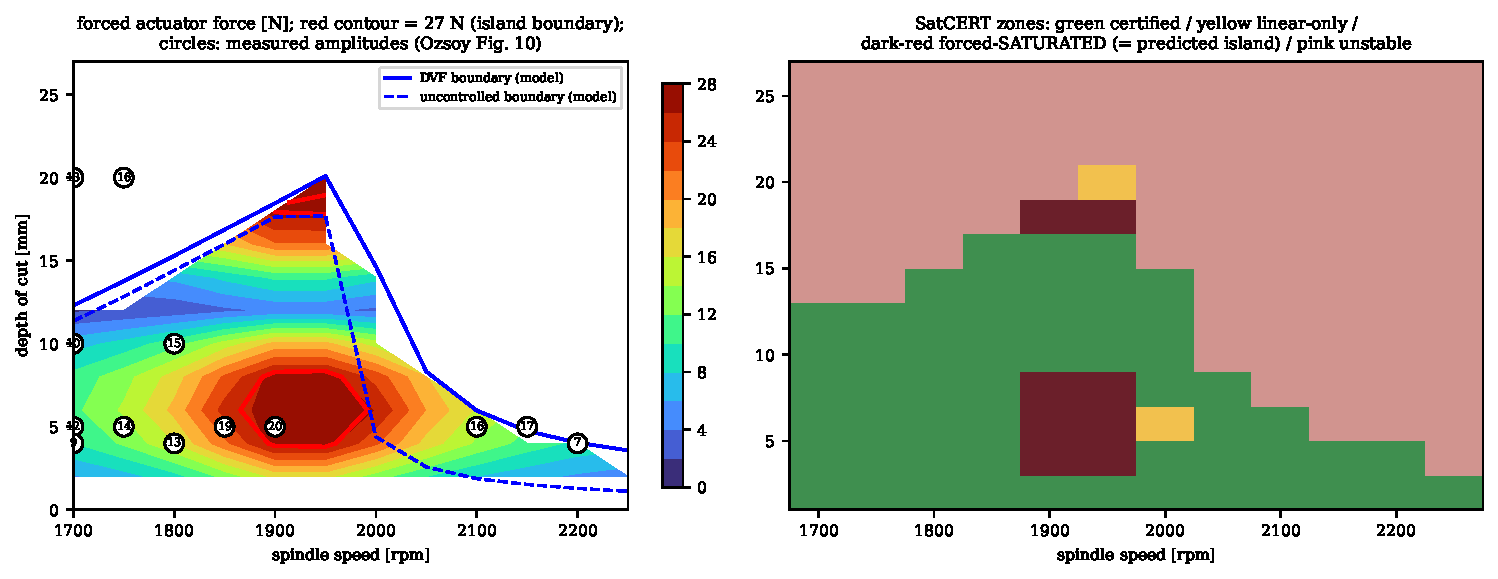
\includegraphics[width=\textwidth]{figures/ozsoy_reproduction}
\caption{Reproduction of the published saturation islands on the
published parameters. Left: forced actuator-force map with the 27\,N
island contour and the measured amplitudes of \cite{ozsoy2025mssp}
(circles). Right: certificate zones; the forced-saturated zones are
the predicted islands.}
\label{fig:ozsoy}
\end{figure}

\begin{itemize}
\item the forced actuator-force amplitudes match the thirteen
measured values printed in the paper's island figure at a median
model/measured ratio of \textbf{1.04} (cell-wise within
$\sim\pm30$\%, consistent with the untabulated edge coefficients,
measured runout, and the single-mode reduction);
\item \emph{both} published islands appear in place as the
certificate census's forced-saturated zones --- the central island at
1900--1950\,rpm\,/\,4--8\,mm and the upper island at $\sim$18\,mm ---
with the saturation-free region between (10--16\,mm) that the paper
highlights; the paper's third band of marginal-chatter cells at
2050--2250\,rpm lies along the model's stability boundary, as
described there;
\item causal probes at the central island run at 44.6\% clip duty
with mildly degraded RMS and no chatter, matching the paper's
``saturated (marginal)'' designations.
\end{itemize}

The reproduction also settles the mechanism: the published islands
are \emph{forced-response} saturation of a mode lying \emph{inside}
the tooth-passing band (128.1\,Hz; the first harmonic resonates at
1921\,rpm, the measured island center) --- exactly the
forced-saturated zones our machinery predicts, with regeneration
included where the published frequency-domain model omits it. A
class-representative counterfactual with the mode \emph{below} the
band (25\,Hz vs.\ 100--200\,Hz forcing) produced \emph{no} island up
to matched clipping depths where the plate's scheduled \hinf{}
latched into chatter: a clipped velocity feedback still outputs a
dissipative $-\dot x$-signed force, whereas a clipped high-gain
model-based loop loses its stabilizing phase. Island susceptibility
is therefore set not by clipping depth but by the \emph{phase
integrity of the clipped feedback} and the spectral placement of the
dominant mode --- a design-relevant conclusion beyond certification.

%% ====================================================================
\section{Discussion and limitations}
\label{sec:discussion}

The certificates delivered here refuse clipping rather than exploit
it; Section~\ref{sec:satregime} shows that above the open-loop
boundary this is not a weakness but the only option for
sector-global guarantees, and quantifies the conservatism against
true basins (20--3100$\times$ at the island points). All certificates
are nominal-model and deterministic: robustness to
cutting-coefficient dispersion and modal tolerance is assessed
statistically in the companion campaign \cite{companion}; sensor
noise is excluded from the certificate and present in the evaluation
simulations. The SDOF reproduction carries declared reductions
(single mode, no edge coefficients, no runout, assumed feedback
rate, one calibrated sign). The tolerance-resolved ranking of
Table~\ref{tab:ranking} is specific to this benchmark and controller
family; its methodological point --- that linear margins can misrank
controllers under saturation, and that the certified ranking depends
on the declared tolerance --- is general, and we propose the
tolerance-resolved certified envelope as the object that active
chatter control papers should report alongside stability lobes.

%% ====================================================================
\section{Conclusions}
\label{sec:conclusions}

(1)~An implementation-exact, solver-free regional certificate for
saturated active chatter control was constructed from the maximal
output admissible set of a sampled-data period lifting, validated to
0.01--1.8\% against an independent nonlinear simulator's measured
clip onset. (2)~Sweeping it yields tolerance-resolved certified
envelopes under which the linear controller ranking collapses
(3.2$\times$ $\to$ 1.32$\times$) and inverts (0.79$\times$ at
20\um) --- saturation certification changes which controller wins.
(3)~Two saturation islands were demonstrated with causal attribution
to the amplifier bound, and the certificate quantifies its own
conservatism against them. (4)~In the saturated regime, a structural
impossibility result scopes what any global certificate can promise
above the open-loop boundary, and a certified negative result shows
classic back-calculation anti-windup cannot improve the
circle-criterion level for either design. (5)~The published
saturation islands of \cite{ozsoy2025mssp} were reproduced
quantitatively on their published parameters (median forced-force
ratio 1.04; both islands in place), unifying their frequency-domain
saturation model with the present certificates and isolating the
island mechanism: forced-response saturation of a mode inside the
tooth-passing band, aggravated by loss of phase integrity of the
clipped feedback.

%% ====================================================================
\section*{Data availability}
The complete model, certificates, campaigns, and every number in this
paper are reproducible from the repository accompanying the
manuscript (scripts and machine-readable records referenced
throughout).

\bibliographystyle{elsarticle-num}
\bibliography{refs}

\end{document}
